\documentclass{article}
\usepackage{hyperref}
\usepackage{amsmath} % or simply amstext
\newcommand{\angstrom}{\textup{\AA}}

\title{Physical Chemistry Problems and Why We Care}
\usepackage{Sweave}
\begin{document}
\Sconcordance{concordance:Chemistry1.tex:Chemistry1.Rnw:%
1 6 1 1 0 54 1 1 2 1 0 2 1 5 0 1 1 6 0 1 2 22 1 1 2 1 0 1 1 6 0 1 2 89 %
1 1 2 1 0 3 1 1 2 1 1 3 0 2 2 7 0 2 1 4 0 1 2 18 1 1 2 1 0 2 1 6 0 2 1 %
4 0 1 2 17 1}

\maketitle

\section{Introduction}

There are several concepts in \emph{physical chemistry}, i.e. the physics of atoms and chemical properties, that turn out to have wide applications and we are going to explore some of them here. 

First, we should acknowledge that the early history is filled with people who had the luxury to explore rather esoteric topics, while we might be learning these as a matter of our own `development' and with a sense of what for!  I'll try to make an argument that this stuff really does matter, but for now, let's start the problem set!

Second, we also need to understand that these assignments have been developed as hurtles that have almost nothing to do with the end-goal of being a health-care professional. Instead, it's better to reflect that being able to think about problem solving is actually the real goal here and we need to learn to problem solve in a systematic way.


\section{Problem Sets}

\begin{figure}
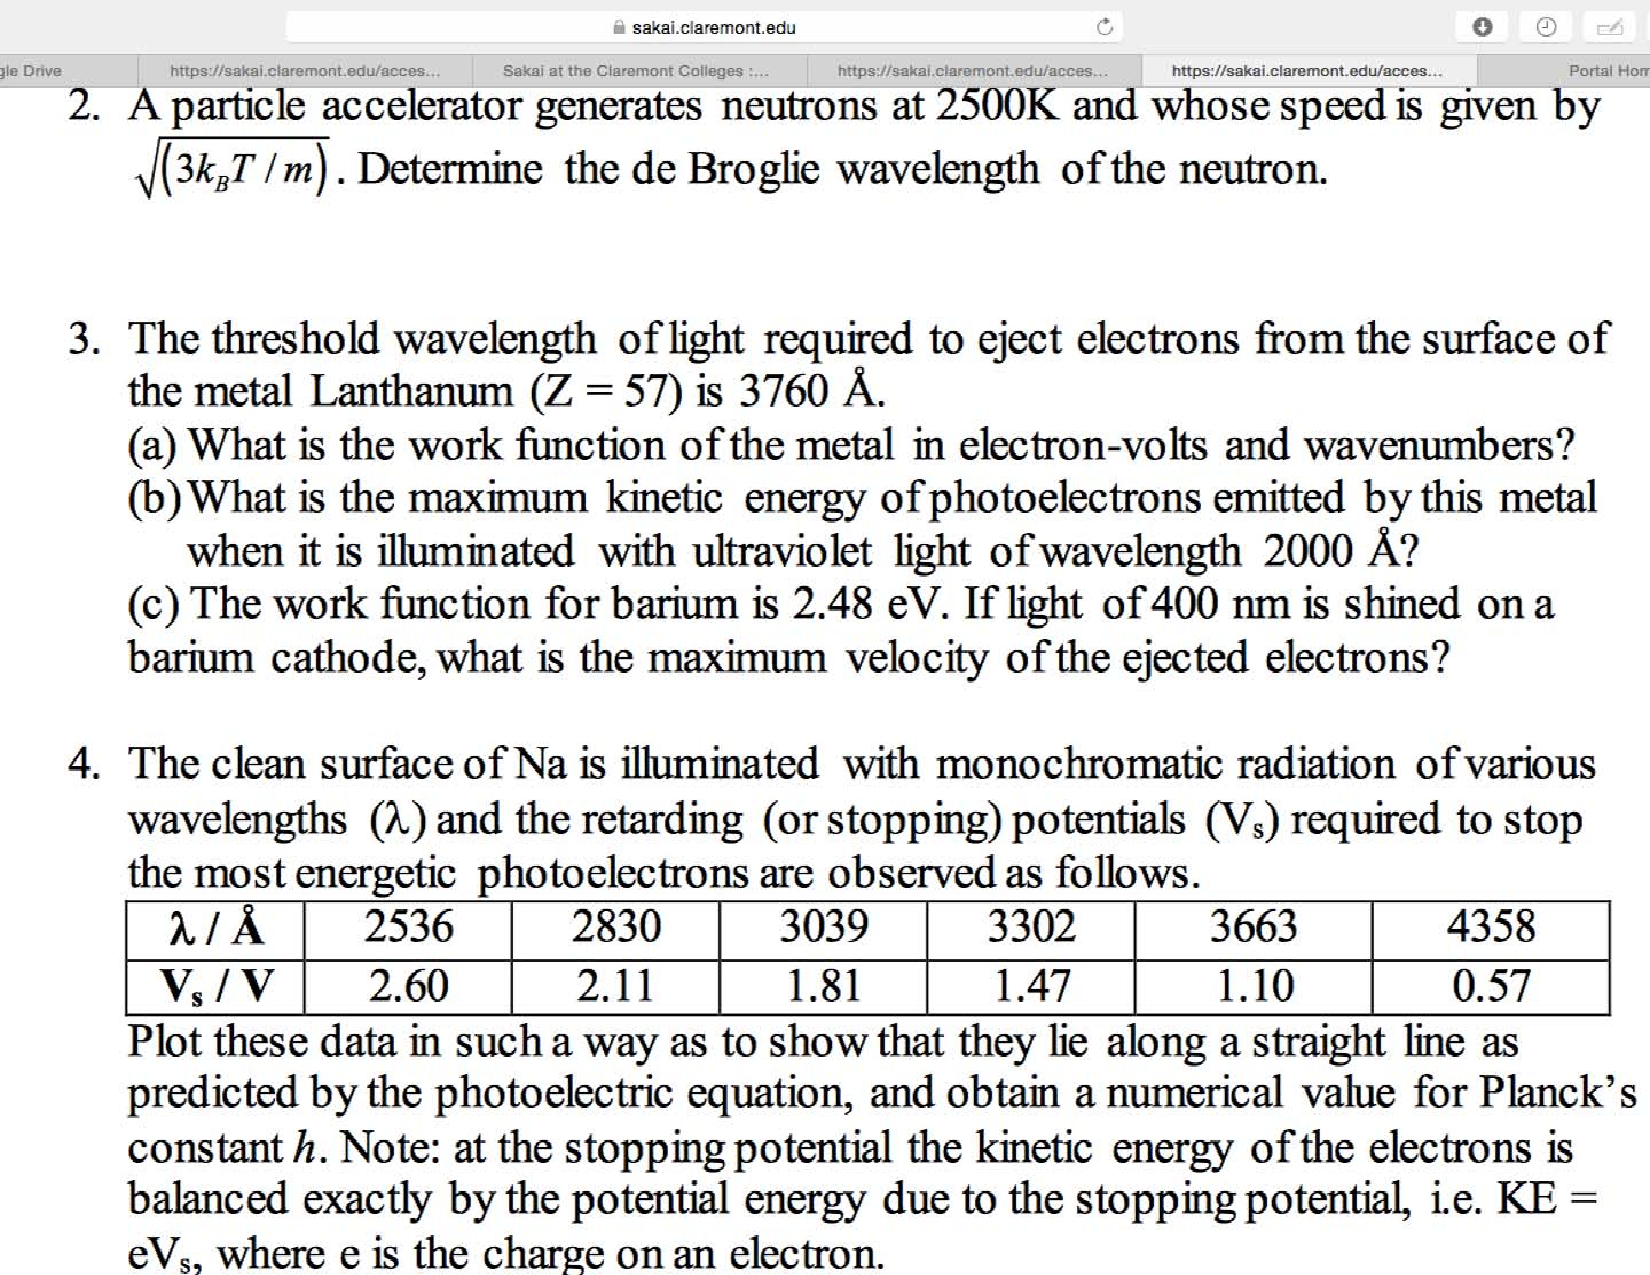
\includegraphics{ProblemSet}
\end{figure}

\section{Problem \#2}

\subsection{Background}
Neutron radiation is a kind of ionizing radiation which consists of free neutrons. A result of nuclear fission or nuclear fusion, it consists of the release of free neutrons from atoms, and these free neutrons react with nuclei of other atoms to form new isotopes, which, in turn, may produce radiation.

Cold, thermal and hot neutron radiation is most commonly used for scattering and diffraction experiments in order to assess the properties and the structure of materials in crystallography, condensed matter physics, biology, solid state chemistry, materials science, geology, mineralogy and related sciences. Neutron radiation is also used in select facilities to treat cancerous tumors due to its highly penetrating and damaging nature to cellular structure. Neutrons can also be used for imaging of industrial parts termed neutron radiography when using film, neutron radioscopy when taking a digital image, such as through image plates, and neutron tomography for three-dimensional images. Neutron imaging is commonly used in the nuclear industry, the space and aerospace industry, as well as the high reliability explosives industry.

The imaging is a function of the particles wavelength, $\lambda$, where higher freqencies resolve higher resolution. It's rare that one would ever have to calculate this from scratch, but the value of the exercise is ??? 

\subsection{de Broglie Wavelenth}

In 1923, Louis de Broglie, a French physicist, proposed a hypothesis to explain the theory of the atomic structure. By using a series of substitution de Broglie hypothesizes particles to hold properties of waves. Within a few years, de Broglie's hypothesis was tested by scientists shooting electrons and rays of lights through slits. What scientists discovered was the electron stream acted the same was as light proving de Broglie correct.

Thus, for this problem, we will determine the wavelength of a particle (nuetron), which also has a mass -- one of the strangest scientific theories!

In this problem we are trying to determine (calculate) the `de Brogie' wavelenth. So, let's first determine the units of a wavelength, so we have a clue where we are heading!  In general, wavelength is measured as length per time, in SI units, we often see this as m/s, but for atomic particle scales, the units are often \angstrom/second, where an Angstrom (\angstrom) is $1 \cdot  10^{-10}$ meters, i.e very short disances! Note: an \angstrom~ is not an SI unit, which is terribly lame. But let's let that go for now, I think $1\cdot 10^{-9}$ is the SI units, which is a nanometer.  Whatever!

We are given the a number that includes temperature, as measured in Kelvin. Okay, that seems to be a weird parameter to be given! But let's back up. We are told that a particle accelartor generate nuetrons at 2500K, where K is degrees Kelvin, i.e. a temperature. By knowing temperature, we are supposed to figure out a wavelength, weird!!!

We are given the following equation to determine velocity of the nuetron

\begin{equation}
v_{rms} = \sqrt{(3k_BT/m)}
\end{equation}

where $v_{rms}$ is room-mean-speed (m/s), $k_B$ is Boltzmann's Constant ($1.38e^{-23}$ J/K or $m^2kg s^{-2} K{-1}$) and T is temperature (degrees K) and m is the mass of the particle (kg). This equation is the root-mean square of speed (velocity) of particles -- it's a kind of an average speed, see \url{http://www.studyphysics.ca/2007/20/ap_thermodynamics/42a_ap_kinetic_theory_gases.pdf} for a decent explanation. For now, we'll use $v_{rms}$ as arithmetic mean of the squares of a set of numbers). The RMS is also known as the quadratic mean and is a particular case of the generalized mean with exponent.

The mass of a nuetron, m, is 1.6750e-27 (kg) and $k_B$ = 1.38e-23 ($m^2kg s^{-2} K{-1}$). Using the equation above, we can do a dimensional analysis where

\begin{equation}
\sqrt{3  m^2\cdot kg\cdot s^{-2} \cdot K^{-1} \cdot K/ kg} = \sqrt{3m^2 \cdot s^{-2}} = \sqrt{3}m/s
\end{equation}

\noindent thus, we have units in terms of velocity! 

Thus, the $\nu_{rms}$ is
\begin{Schunk}
\begin{Sinput}
> k_B = 1.38e-23
> T = 2500
> m = 1.6750e-27; m
\end{Sinput}
\begin{Soutput}
[1] 1.675e-27
\end{Soutput}
\begin{Sinput}
> v = sqrt(3*k_B*T/m); v
\end{Sinput}
\begin{Soutput}
[1] 7860.728
\end{Soutput}
\end{Schunk}

Thus, we have now calculated the speed as 7860.73.\footnote{However, I am not sure this is right. Did you get this as a intermediate answer with your prof? I need to figure out the units too!}

\subsection{Calculating $\lambda$}

Next, what do we do with the velocity?  

Using this site: \url{http://chem.libretexts.org/Core/Physical_and_Theoretical_Chemistry/Quantum_Mechanics/02._Fundamental_Concepts_of_Quantum_Mechanics/De_Broglie_Wavelength}, we might be able to evaluate the question with some sense that we understand what in the world is happening:

\begin{equation}
\lambda = \frac{h}{p} = \frac{h}{ m v}
\end{equation}

\noindent where h is planck's constant, p is the particle momentum and m is the particle's mass and $\nu$ is the particles' velocity. Using a dimensional analysis we have

\begin{equation}
\frac{m^2 \cdot kg \cdot s^{-1}}{kg \cdot m /s} = m  
\end{equation}

\noindent and we have meters, which is how wavelengths are measured!

Based on this equation, we have velocity, $\nu$, and we know the mass of the nuetron, which is 0. Thankfully, h, or Planck's Constant is a known quanity, altough we derive it in problem \#4!

\begin{Schunk}
\begin{Sinput}
> h = 6.626e-34
> lambda = h /(m * v); lambda
\end{Sinput}
\begin{Soutput}
[1] 5.032385e-11
\end{Soutput}
\end{Schunk}

I calcualted a wavelength that seems small, but might be reasonable, 5.03e-11.\footnote{How does this compare with the answer you calculated?}

\section{On Planck's Constant}

Planck's Constant is a very powerful parameter... with units as $m^2 \cdot kg \cdot s^{-1}$. 

For background on Planck's constant, check out \url{https://en.wikipedia.org/wiki/Planck_constant}. 

\subsection{Stopping Voltage and Wavelength}

The goals of this problem is to determine the constant using stopping voltages for various wavelengths. I am not sure how this is done, for now, let's say in a fancy machine and leave it at that.

The real value of this experiment is it allows physicist to estimate Planck's Constant, which is used to calculate a range of physical and chemical processes, for example the speed of light!

We given a table to measurements: 
\begin{itemize}
\item $\lambda/\angstrom$ is in the units of lenth and in this case is is in \angstrom, or Angstroms. Unfortunately, the symbolism is non-standard here, where it looks like we are dividing the wavelength by the \angstrom, but after several attempts to use the demominator, I discoverd that it was only referring to the units. 

\item $V_s/V$ is the stopping voltage, but the demominator is confusing, and is again referring to the units, which are in volts!
\end{itemize}

We are told to create a line, but the predicted by the photoelectric equation. There are several versions of the equation, e.g.,

\begin{equation}
E = h \cdot \nu
\end{equation}

\noindent E or $\nu$ are not given. 

Alternatively, we might calculate the maximum energy of an electron ejected,

\begin{equation}
K_{max} = h \cdot \nu - \phi
\end{equation}

\noindent where $\nu$ is the frequency, $\phi$ is the work function, h is Plank's constant. 

So, we'll need to figure out how to manipulate our equation for parameters we have measured. 

This equation was proposed by Einstein -- where energy is proporation to freqency and h. Now, first, there is something that is tricky about this equation, where frequency is often denoted as $\nu$, which is not the same as v used for velocity as above. This is an annoying part of science, there just aren't enough letters for them to represent one thing and even worse many of them look a like! So, you have to be careful. 

According to wikipedia, E is a work function. I am not sure what that means, so, for now, we'll let then be -- perhaps it will be clear later!

Using a dimensional analysis, where frequency is $s{-1}$, we obtain

\begin{equation}
m^2 \cdot kg \cdot s^{-1} \cdot s^{-1} = kg m^2 s^{-2} = Joule
\end{equation}

\noindent the units as espected is a joule. 

Next, we can convert wavelength (m) to frequency (s) using this simple equation:

\begin{equation}
\nu = \frac{v}{\lambda}
\end{equation}

\noindent, now however, we need to figure out the v, velocity!  Dang!  Another set of steps. 

For now, let's do some substuting and see where we end up: 

\begin{equation}
E = h \nu = h \frac{v}{\lambda}
\end{equation}

Now, we to deal with E. It's not clear what this is really in relation to the equation below, perhaps, KE = E? For now, I'll assume that, but from what I have read there isn't any reason that I can make that assumption.

\begin{equation}
KE = e \cdot V_s 
\end{equation}

\noindent where KE is kenetic energy (units?) and E is the charge of an electron (volts) and $V_s$ is stopping voltage. KE is $1/2 mv^2$. e is the charge of an electron. Let's start with a simple approach:

\begin{equation}
KE = e \cdot V_s = h \frac{v}{\lambda}
\end{equation}
 
\begin{equation}
e \cdot V_s \cdot v = h \lambda
\end{equation}

I suspect this is the velocity of light -- of course, light's speed will vary with what is travels through and we are not given that information. Bummer. Perhaps, we can assume it's traveling through a vacuum... where v = 299792458 meters per second. e is the charge of an electron, which is measured in Coulumbs, 1.602e-19. 

Using dimensional analysis then we have 

\begin{equation}
columbs \cdot volts
\end{equation}

\begin{Schunk}
\begin{Sinput}
> e = 1.602e-19
> v = 299702458
> lambda=c(2536, 2830, 3039, 3302, 3663, 4358)
> Vs=c(2.6, 2.11, 1.81, 1.47, 1.1, .57)
> left = Vs * e * v 
> right = lambda
\end{Sinput}
\end{Schunk}

\begin{Schunk}
\begin{Sinput}
> coef(lm(left~right))
\end{Sinput}
\begin{Soutput}
  (Intercept)         right 
 2.505048e-10 -5.267790e-14 
\end{Soutput}
\begin{Sinput}
> plot(left~right)
> abline(coef(lm(left~right)))
\end{Sinput}
\end{Schunk}
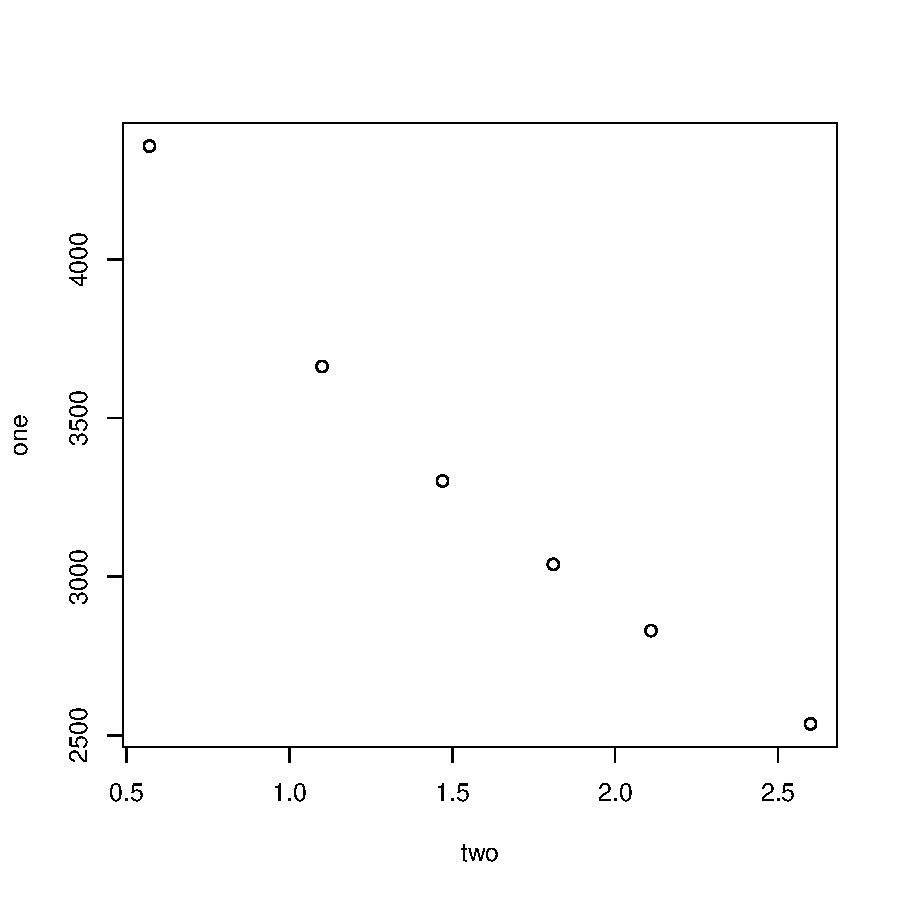
\includegraphics{Chemistry1-004}

and then e =mc2?  somehow we need to involve the speed of light? Geez, I am completely lost!



Alternatively, we can substitute E, from the photoelectric equation:

\begin{equation}
KE = \cdot h \cdot freq \cdot V_s
\end{equation}

and solving for h, we get

\begin{equation}
h = freq \cdot V_s /KE
\end{equation}

Here, I am stuck again...

\begin{Schunk}
\begin{Sinput}
> lambda=c(2536, 2830, 3039, 3302, 3663, 4358)
> volts=c(2.6, 2.11, 1.81, 1.47, 1.1, .57)
> coef(lm(lambda~volts))
\end{Sinput}
\begin{Soutput}
(Intercept)       volts 
  4713.1565   -885.1904 
\end{Soutput}
\begin{Sinput}
> plot(lambda~volts)
> abline(coef(lm(lambda~volts)))
\end{Sinput}
\end{Schunk}
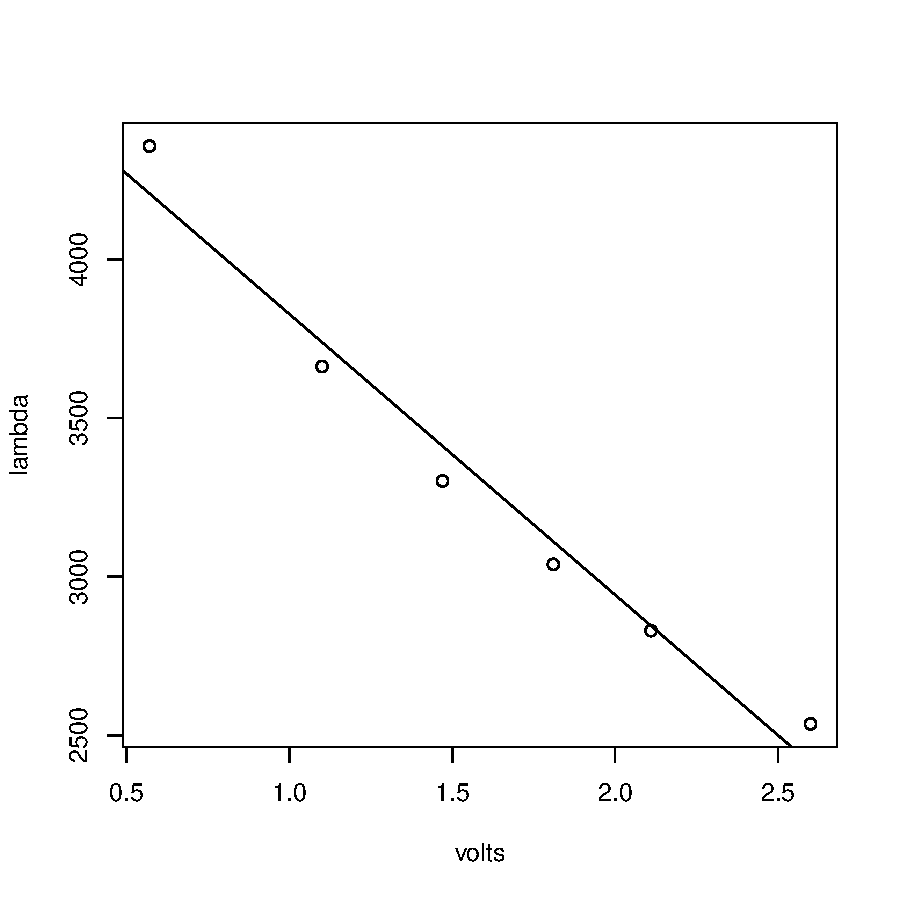
\includegraphics{Chemistry1-005}

The the slope is not h!  where h is 4713.16, based on the relationship:

\begin{equation}
\lambda = f(V_s)
\end{equation}

This doesn't seem to be doing anything useful. 

\noindent where E is the energy of the radiation and $\nu$ is the velocity of the particle. 







\end{document}
